\documentclass[12pt]{article}
%\usepackage[utf8]{inputenc}
%\documentclass[UTF8]{ctexart}
%\usepackage[UTF8, heading = false, scheme = plain]{ctex}
\usepackage{geometry}
%geometry{a4paper,scale=0.9}
\geometry{a4paper,left=1cm,right=1cm,top=1cm,bottom=2cm}
\usepackage{amsfonts}
\usepackage{color}
\usepackage{url}
%\usepackage{biblatex}
\usepackage{amsmath}
\usepackage{amssymb}
\usepackage{latexsym}
\usepackage{cite}
%\addbibresource{ref.bib}
%\bibliography{ref.bib}
\usepackage{caption}
\usepackage{graphicx, subfig}
\usepackage{float}
%\usepackage[fontset=ubuntu]{ctex}
%\usepackage{fontspec}
\usepackage{xeCJK}
%\usepackage[colorlinks,
%anchorcolor=black,
%citecolor=black]{hyperref}
%\setmainfont{SimSun}
\usepackage[section]{placeins}
\usepackage{enumitem}
\usepackage{framed}
\usepackage[framemethod=TikZ]{mdframed}
\usepackage{indentfirst}
\usepackage{setspace}%使用间距宏包
\linespread{1.5}

\title{群论的预备知识\cite{From_Linear_Equation_To_Galois_Theory}}
\author{leolinuxer}
%\date{June 2020}

\begin{document}
%\setlength{\parindent}{0pt}
\maketitle
\tableofcontents

\section{集合与映射}
\subsection{集合基本概念}
\begin{itemize}
\setlength{\itemsep}{0pt}
\setlength{\parsep}{0pt}
\setlength{\parskip}{0pt}
    \item \textbf{并集}:$C = A\cup B$,即$x\in C \Leftrightarrow x\in A \quad or \quad x \in B$
    \item \textbf{交集}:$C = A \cap B$,即$x\in C \Leftrightarrow x\in A \quad \& \quad x \in B$
    \item \textbf{差集}:$C = A - B$,即$x\in C \Leftrightarrow x\in A \quad \& \quad x \notin B$
    \item \textbf{直积}:$C = A \times B = \{(a,b)|a\in A \& b \in B\}$
\end{itemize}

若映射$f: A \rightarrow B$有如下不同情况,可以区分出:

1) 若$A \subset B$,而$f$满足$f(a) = a, \forall a \in A$,则称$f$为\textbf{包含映射},记为$i$;若此时 $B=A$,此时的 $i$ 称为$A$的\textbf{恒等映射},记作$1_A$。

2) 若$f(A) = B$,则称$f$为\textbf{$A$到$B$的满射}

3) 若 $f(a) = f(a') \Rightarrow a = a', a,a \in A$,则称 $f$ 为\textbf{单射}。

4) 若$f$ 既是单射又是满射,则称$f$为\textbf{双射};此时从 $f(a) = b$,可记$a = f^{-1}(b)$,从而确定了映射$f^{-1}: B \rightarrow A$,称为$f$的\textbf{逆映射}。

5) 若$C \subset A$,则由于$f(c) \in B$ 对应于$c \in C$,可定义$f_c: C \rightarrow B$,即把$f$的定义域缩小到$C$上,则称$f_c$为$f$到$C$的\textbf{限制}。

\begin{framed}
%\verb|\documentstyle[ifthen,12pt,titlepage]{article}|
如果$f: A \rightarrow B$,且$g: B \rightarrow C$,此时把$a \in A$映为$h(a) = g(f(a)) \in C$ 来定义映射$h: A \rightarrow C$,则称$h$为$f$和$g$的\textbf{结合},记作$h = g\circ f$

如果$f: A \rightarrow B$是双射,不难看出$f^{-1}: B \rightarrow A$也是双射,且 $f^{-1}\circ f = 1_A, f\circ f^{-1} = 1_B$

对于$f: A \rightarrow B, g: B \rightarrow C, h: C \rightarrow D$,有$h\circ (g\circ f) = (h\circ g)\circ f$,即映射的结合运算满足结合律。
\end{framed}


\subsection{集合$A$中的变换}
考虑$f: A \rightarrow B$,且$B = A$,即\textbf{$f$是$A$到$A$自身的映射,把映射$f$称为$A$的一个变换},即$f$将$a \in A$变为$f(a) \in A$。

\textbf{$A$的所有变换,构成集合$T$,称为$A$的变换全集}。

\textbf{$A$的所有双射构成$T$的一个重要子集,记作$G$,称为$A$的变换群}。集合$G$具有如下性质:

1) $1_A \in G$,即$G$中含有\textbf{恒等变换}。

2) $f \in G \Leftrightarrow f^{-1} \in G$

3) $f \in G, g\in G \Rightarrow g \circ f \in G$。因此$G$的元素对结合运算$\circ$而言是\textbf{封闭的}。

4) 对于$f, h, h \in G$,可知$(h \circ g) \circ f = h \circ( g \circ f)$,即 $G$ 的元素对 $\circ$ 满足结合律。

\begin{framed}
%\verb|\documentstyle[ifthen,12pt,titlepage]{article}|
\small {
思考:$T$包含$A$的\textbf{所有}变换,其中包括从$A$到$A$的双射(一一映射),也包括其它变换;而$A$的所有\textbf{双射}(一一映射)构成的$T$的子集$G$,也就是$A$的变换群;
}
\end{framed}

\subsection{关系、等价关系与分类}
\subsubsection{关系}
映射反应的是一个集合与另一个集合的外部联系;“关系”给出了集合内元素的内部联系。

集合上的一个\textbf{关系$\sim$},指的是一种法则。由它可以判断任意$a,b\in A$所构成的有序偶$(a,b)$ 是满足某种条件(此时称$a,b$有关系,记作$a\sim b$),还是不满足这一条件(此时称$a,b$无关系,记作$a\nsim b$)

\begin{framed}
%\verb|\documentstyle[ifthen,12pt,titlepage]{article}|
\small {
例如大于($\ge$)就给出了整数集合$Z$的一个关系;对于三角形的集合,三角形的全等和相似也分别给出了这个集合的一个关系。
}
\end{framed}

\subsubsection{等价关系}
集合$A$上定义的关系$\sim$,若满足如下条件,则称$\sim$是一个等价关系:

1) 自反律:对$\forall a \in A \Rightarrow a \sim a$

2) 对称率:对$a \sim b \Rightarrow b \sim a$

3) 传递率:对$a \sim b, b \sim c\Rightarrow a \sim c$

\subsubsection{集合的分类}
集合$A$的一个\textbf{分类},指的是把$A$分成许多称为\textbf{类}的非空子集合$A_a, A_b, \cdots $,而其中每两个不同类的交集为空集,它们全体的并集是$A$。

设$\sim$是集合$A$的一个等价关系,对于$a\in A$,我们把$A$中所有与$a$等价的元都汇集在一起,而构造出$A$的子集合$A_a$,如果此时存在$b \in A$,且 $b \notin A_a$,则同样构造$A_b$,显然这些$A_a, A_b, \cdots $给出$A$的一个分类。

反过来,如果给定了$A$的一个分类,那么我们就可以如下的定义$A$的一个等价关系:$\sim: a \sim b$,当且仅当$a,b$属于同一类;$a \nsim b$,当且仅当$a,b$不属于同一类;

总结后有:集合$A$的一个分类可以确定它的一个等价关系;反之,集合$A$的一个等价关系可以确定它的一个分类。

因此,类也称为\textbf{等价类}。而$A_a$称为\textbf{由$a$确定的等价类}, $a$是$A_a$的一个\textbf{代表}。当然,若$a \sim b$,则$A_a = A_b$,即一个等价类可以由其中的任一元做代表,因为有这种随意性,所以任何关于等价类的命题首先必须与\textbf{代表元的选取无关}。

\begin{framed}
%\verb|\documentstyle[ifthen,12pt,titlepage]{article}|
\small {
全体奇数和全体偶数这两个集合构成了整数集合$Z$的一个分类。

理解:集合的分类是\textbf{不重不漏}的。
}
\end{framed}

\subsubsection{商集合}
由$A$的等价关系$\sim$,确定了$A$的各个类$A_a, A_b, \cdots$,以这些类做为元素而得到的集合,称为由$A$按$\sim$而确定的商集合,记作:
$$
A / \sim = \{A_a, A_b, \cdots \}
$$

此时,很自然的由$a$对应$A_a$,可定义$f: A \rightarrow A/\sim$,容易验证这是一个满射,称为$A$到商集合$A/\sim$上的\textbf{自然映射}。

\subsection{整数集合$Z$与同余关系}
接下来,我们把上面的理论应用到整数集合$Z$上。取定$n\in N^*$,定义关系$\sim: a \sim b$,当且仅当$a-b$能被$n$整除时(记作$n|(a-b)$),称$a,b$对于\textbf{模$n$同余},记作$ a \equiv b\quad mod(n)$。

可以证明,这是一个等价关系;这时的等价类称为模$n$的\textbf{同余类};通常把以$a$为代表的同余类记作$[a]_n$或简记为$[a]$或$\bar{a}$。而把此时的商集合记为$Z_n$,称为\textbf{模$n$同余类集合}。于是:
$$
\bar{a} = \{a + kn\ | k \in Z\}
$$
$$
Z_n = \{\bar{1}, \bar{2}, \cdots, \bar{n}\}
$$

\begin{framed}
%\verb|\documentstyle[ifthen,12pt,titlepage]{article}|
\small {
举例:

当$n=2$时,模2同余的数分别为$\{1, 3, 5, \cdots\}$和$\{2, 4, 6, \cdots, \}$。因此$Z_2 = \{\bar{1}, \bar{2}\}$;其中$\bar{1}$为全体奇数,$\bar{2}$为全体偶数;

当$n=7$时,$Z_7 = \{\bar{1}, \bar{2}, \bar{3}, \bar{4}, \bar{5}, \bar{6} \}$;对于一年中的365天,这些同余类通常以周一、周二、……、周日来标记。同理,对于年份,可以按$n=12$划分为以十二生肖为代表的12个同余类。
}
\end{framed}

为了今后的应用,我们在$Z_n$中再划分出一个重要的子集$Z'_n$来。为此,对于$l, m \in N^*$,我们以$(l, m)$来表示$l, m$的最大公因数。如果$l, m$互素,则$(l,m)=1$。定义:
$$
Z'_n = \{\bar{k} \in Z_n | 1 \le k \le n, (k,n) = 1\}
$$
称为\textbf{模$n$同余类乘群}。

\begin{framed}
%\verb|\documentstyle[ifthen,12pt,titlepage]{article}|
\small {
举例:当 $n=6$时,$Z_6 = \{\bar{1}, \bar{2}, \bar{3}, \bar{4}, \bar{5}, \bar{6}\}$,其中与$n=6$互素的元素为$\bar{1}, \bar{5}$,所以$Z'_6 = \{\bar{1}, \bar{5}\}$;
}
\end{framed}

当$p$是素数时,有$Z_p = \{\bar{1}, \bar{2}, \cdots, \overline{p-1}, \bar{p}\}$,$Z'_p = \{\bar{1}, \bar{2}, \cdots, \overline{p-1} \}$

\begin{framed}
%\verb|\documentstyle[ifthen,12pt,titlepage]{article}|
\small {
举例:当 $n=17$时,$Z'_{17} = \{\overline{1}, \overline{2}, \overline{3}, \overline{4}, \overline{5},\cdots, \overline{16}\}$;而数$3^m$,对 $m = 0, 1, 2, \cdots, 15$ 所属的同余类分别为:
\begin{itemize}
\setlength{\itemsep}{0pt}
\setlength{\parsep}{0pt}
\setlength{\parskip}{0pt}
    \item $m=0$时,$3^m = 1$所属的同余类为$\overline{1}$
    \item $m=1$时,$3^m = 3$所属的同余类为$\overline{3}$
    \item $m=2$时,$3^m = 9$所属的同余类为$\overline{9}$
    \item $m=3$时,$3^m = 27$所属的同余类为$\overline{10}$
    \item $\cdots$
\end{itemize}

\textbf{即数$3^m$,对 $m = 0, 1, 2, \cdots, 15$ 所属的同余类分别为:$\overline{1}, \overline{3}, \overline{9}, \overline{10}, \overline{13}, \overline{5}, \overline{11}, \overline{16}, \overline{14}, \overline{8}, \overline{7}, \overline{4}, \overline{12}, \overline{2}, \overline{6}$,它们是$\bar{1}, \overline{2}, \overline{3}, \overline{4}, \overline{5},\cdots, \overline{16}$的另一种排列。}
}
\end{framed}

\subsection{算数基本定理与欧拉函数$\varphi(n)$}
欧拉函数$\varphi(n)$的定义为 $Z'_n$中元素的个数。即$\varphi(x)$等于满足$1\le k \le n$,及$(k,n)=1$的正整数$k$的个数。

根据定义,显然有:$\varphi(1) = \varphi(2) = 1, \varphi(3) = \varphi(4) = \varphi(6) = 2, \varphi(5) = 4, \cdots$

\begin{framed}
%\verb|\documentstyle[ifthen,12pt,titlepage]{article}|
\small {
证明如下:

$ Z'_1 = \{\bar{1}\}, Z'_2 = \{\bar{1}\} \Rightarrow \varphi(1) = \varphi(2) = 1 $

$ Z'_3 = \{\bar{1}, \bar{2}\}, Z'_4 = \{\bar{1}, \bar{2}\}, Z'_6 = \{\bar{1}, \bar{5}\} \Rightarrow \varphi(3) = \varphi(4) = \varphi(6) = 2 $

$ Z'_5 = \{\bar{1}, \bar{2}, \bar{3}, \bar{4}\} \Rightarrow \varphi(5) = 4 $
}
\end{framed}

为了推导$\varphi(n)$的计算公式,我们先来叙述\textbf{算数基本定理}。因为任何大于1 的整数$n$都或是合数或是素数。而如果$n$是合数,则$n$可以唯一地分解为一系列素数的乘积,这就是:

\begin{mdframed}[
linecolor=black!40,outerlinewidth=1pt,roundcorner=.5em,innertopmargin=1ex,innerbottommargin=.5\baselineskip,innerrightmargin=1em,innerleftmargin=1em,backgroundcolor=gray!5,
%backgroundcolor=blue!10,%userdefinedwidth=1\textwidth,%shadow=true,%shadowsize=6,%shadowcolor=black!20,%frametitle={The \textit{two-step} model of XMCD:},%frametitlebackgroundcolor=cyan!40,%frametitlerulewidth=10pt
]
\textbf{算数基本定理}:对于大于1的自然数,一定可把它唯一地表达为$n = p_1^{v_1} \cdot p_2^{v_2} \cdot \cdots \cdot p_k^{v_k}$,这里$p_1, p_2, \cdots, p_k$是素数,且$v_1, v_2, \cdots, v_k \in N^*$。
\end{mdframed}

为了求得$\varphi(n)$的表达式,先来讨论两个简单的情况,再把它们综合起来:

1) 首先求$\varphi(p^n)$,这里$p$是素数。对于$1 \le k \le p^n$的$k$,要与$p^n$互素,其充要条件是$k$不能被$p$整除,即$p \nmid k$。然而,在$1$到$p^n$之间,有 $p^{n-1}$ 个数,即$p, 2p, 3p, \cdots, (p^{n-1}p)$是能被$p$整除的,因此其中不能被$p$整除的数共有$p^n - p^{n-1}$个。于是有:

\begin{mdframed}[
linecolor=black!40,outerlinewidth=1pt,roundcorner=.5em,innertopmargin=1ex,innerbottommargin=.5\baselineskip,innerrightmargin=1em,innerleftmargin=1em,backgroundcolor=gray!5,
%backgroundcolor=blue!10,%userdefinedwidth=1\textwidth,%shadow=true,%shadowsize=6,%shadowcolor=black!20,%frametitle={The \textit{two-step} model of XMCD:},%frametitlebackgroundcolor=cyan!40,%frametitlerulewidth=10pt
]
\textbf{定理:设$p$是一个素数,则
$$
\varphi(p^n) = p^n(1 - \frac{1}{p})
$$
特别的,当$n=1$时,$\varphi(p) = p - 1$。}
\end{mdframed}

2)然后,我们设$(l,m)=1$,来求$\varphi(lm)$的计算公式。为此,我们以$[k]_{lm}$映为$([k]_l, [k]_m)$来定义对应:
$$
\rho: Z'_{lm} \rightarrow Z'_l \times Z'_m
$$

不难证明,这一对应是与同余类代表的选取无关的,因此,$\rho$是一个映射。同样也不难证明,$\rho$既是单射又是满射,即是双射。于是$Z'_{lm}$中元素的个数$\varphi(lm)$等于$Z'_l \times Z'_m$中元素的个数,即$Z'_l$中的元素个数
$\varphi(l)$与$Z'_m$中的元素个数$\varphi(m)$的乘积,这就有:

\begin{mdframed}[
linecolor=black!40,outerlinewidth=1pt,roundcorner=.5em,innertopmargin=1ex,innerbottommargin=.5\baselineskip,innerrightmargin=1em,innerleftmargin=1em,backgroundcolor=gray!5,
%backgroundcolor=blue!10,%userdefinedwidth=1\textwidth,%shadow=true,%shadowsize=6,%shadowcolor=black!20,%frametitle={The \textit{two-step} model of XMCD:},%frametitlebackgroundcolor=cyan!40,%frametitlerulewidth=10pt
]
\textbf{
定理:若$(l,m) = 1$,则$\varphi(lm) = \varphi(l) \cdot  \varphi(m)$
}
\end{mdframed}

\begin{framed}
%\verb|\documentstyle[ifthen,12pt,titlepage]{article}|
\small{
待加深理解:注意$(l,m)=1$,即 $l,m$是互素的。然后呢?

举个例子:
$Z'_{15} = \{\overline{1}, \overline{2}, \overline{4}, \overline{7}, \overline{8}, \overline{11}, \overline{13}, \overline{14}\}$
,即$\varphi(15) = 8$

且$15 = 3 \times 5$,$Z'_3 = \{\overline{1}, \overline{2}\}, Z'_5 = \{\overline{1}, \overline{2}, \overline{3}, \overline{4}\}$,

所以$\varphi(3) = 2, \varphi(5) = 4$,即$\varphi(8) = \varphi(3) \cdot  \varphi(5) = 8$
}
\end{framed}

综上两点,有如下定理:
\begin{mdframed}[
linecolor=black!40,outerlinewidth=1pt,roundcorner=.5em,innertopmargin=1ex,innerbottommargin=.5\baselineskip,innerrightmargin=1em,innerleftmargin=1em,backgroundcolor=gray!5,
%backgroundcolor=blue!10,%userdefinedwidth=1\textwidth,%shadow=true,%shadowsize=6,%shadowcolor=black!20,%frametitle={The \textit{two-step} model of XMCD:},%frametitlebackgroundcolor=cyan!40,%frametitlerulewidth=10pt
]
\textbf{
定理:对于大于1的自然数$n$,有:
$$
\varphi(n) = \varphi(p_1^{v_1})\cdots\varphi(p_k^{v_k}) = n(1-\frac{1}{p_1})\cdots(1-\frac{1}{p_k})
$$
其中$p_1, p_2, \cdots, p_k$是$n$的各个素因数。
}
\end{mdframed}

\begin{framed}
%\verb|\documentstyle[ifthen,12pt,titlepage]{article}|
\small{
举个例子:
$Z'_{15} = \{\overline{1}, \overline{2}, \overline{4}, \overline{7}, \overline{8}, \overline{11}, \overline{13}, \overline{14}\}$
,即$\varphi(15) = 8$

且$15 = 3^1 \times 5^1$,所以$\varphi(15) = \varphi(3^1)\varphi(5^1) = 15(1-\frac{1}{3})(1-\frac{1}{5}) = 15
\cdot \frac{2}{3} \cdot \frac{4}{5} = 8$
}
\end{framed}

\section{群论基础}
\subsection{群的定义}

\begin{framed}
%\verb|\documentstyle[ifthen,12pt,titlepage]{article}|
\small{
首先给出下面两个例子:

例1:给出集合$A = \{1, -1\}$,并考虑其中元的通常乘法运算,不难看出集合$A$具有如下性质:
\begin{itemize}
\setlength{\itemsep}{0pt}
\setlength{\parsep}{0pt}
\setlength{\parskip}{0pt}
    \item $A$的元在乘法下是封闭的,即对任意$a,b \in A, a\cdot b \in A$
    \item 该乘法满足结合律,即对任意$a,b,c \in A$,有$ a\cdot (b\cdot c) = (a\cdot b)\cdot c \in A$
    \item 有数 1,它对任意$a \in A$,有 $1 \cdot a = a \cdot 1 = a$
    \item 由$1 \cdot 1 = 1, (-1) \cdot (-1) = 1$,可知对于任意$a \in A$,存在$b \in A$,使得$a\cdot b = b\cdot a = 1$
\end{itemize}

例2:给出整数集合$Z$,并考虑其中元的通常加法运算,同样也有:
\begin{itemize}
\setlength{\itemsep}{0pt}
\setlength{\parsep}{0pt}
\setlength{\parskip}{0pt}
    \item $Z$的元在加法下是封闭的,即对任意$a,b \in Z, a+b \in Z$
    \item 该加法满足结合律,即对任意$a,b,c \in Z$,有$ a + (b + c) = (a + b) + c \in Z$
    \item 有数 0,它对任意$a \in Z$,有 $0 + a = a + 0 = a$
    \item 对于任意$a \in Z$,存在$-a \in Z$,使得$a + (-a) = (-a)+ a = 0$
\end{itemize}
}
\end{framed}

尽管这两个例子中的集合不同,而且所考虑的运算也不同,但是它们具有共性:一个集合,一种封闭的运算,还有同样的一些运算性质。于是人们就从这些具体的原型中抽象出它们的共性,从而提出\textbf{抽象群}的概念,然后对抽象群进行研究。

\begin{framed}
%\verb|\documentstyle[ifthen,12pt,titlepage]{article}|
理解:群论也是从变化中抽取出来的不变性(共性)。在其他领域中,有类似的思考过程。比如在线性空间中,不管坐标基如何变化,向量的”长度“不变;在欧式空间和闵氏空间中,两点间的”距离“不随坐标的变化而变化(虽然欧式空间和闵氏空间对于距离的定义不同);比如拓扑学,也是研究在形状不断变化下,物体的拓扑结构具有什么样的不变形。
\end{framed}

\begin{mdframed}[
linecolor=black!40,outerlinewidth=1pt,roundcorner=.5em,innertopmargin=1ex,innerbottommargin=.5\baselineskip,innerrightmargin=1em,innerleftmargin=1em,backgroundcolor=gray!5,
%backgroundcolor=blue!10,%userdefinedwidth=1\textwidth,%shadow=true,%shadowsize=6,%shadowcolor=black!20,%frametitle={The \textit{two-step} model of XMCD:},%frametitlebackgroundcolor=cyan!40,%frametitlerulewidth=10pt
]
\textbf{
群的定义:在非空集合$G=\{a, b, \cdots, \}$中规定元素间的一种运算,称为“乘法”,记作“$\cdot$”(在不会混淆时可以省略去$\cdot$)。如果$G$对“$\cdot$”满足下列4条公理,则称$G$是一个群,记作$(G, \cdot)$,或简单的用 $G$来表示:
\begin{enumerate}
\setlength{\itemsep}{0pt}
\setlength{\parsep}{0pt}
\setlength{\parskip}{0pt}
    \item 封闭性:若$a,b\in G$,则$a\cdot b \in G$;
    \item 结合律:若$a,b,c \in G$,则$(a\cdot b)\cdot c = a\cdot (b \cdot c)$
    \item 单位元:对任意$a\in G$,存在$e \in G$,满足$e \cdot a = a \cdot e = a$,称$e$为$G$的单位元
    \item 逆元:对任意$a \in G$,都有一个逆元,记作$a^{-1}$,满足$a^{-1} \cdot a = a \cdot a^{-1} = e$
\end{enumerate}
}
\end{mdframed}

于是,$A = \{1, -1\}$在通常乘法下成群;$Z$在通常加法下成群;集合$A$的双射全体,在映射的结合运算下成群,即$A$的变换群。

若对任意$a,b \in G$,有$ab = ba$,则称$G$为\textbf{可换群};对于可换群常用”$+$“代替”$\cdot$“,且把此时的单位元称为\textbf{零元},逆元称为\textbf{负元}。如果群$G$仅含$n$个元素,则称它为\textbf{$n$阶群},记作$|G| = n$,这种群是\textbf{有限群},否则是\textbf{无限群}。

\begin{framed}
%\verb|\documentstyle[ifthen,12pt,titlepage]{article}|
对于上一节定义的$Z_n$,可以如下地定义它的元素的乘法:$\overline{a}\cdot \overline{b} = \overline{ab}$
,但是一般来说,$Z_n$不是群,因为$\overline{n}$没有逆元;不难证明,$\overline{k}$有逆元的充要条件是$(k,n) = 1$,因此$Z'_n$是群,即\textbf{模$n$同余类乘群},它是可交换群,且$|Z'_n| = \varphi(n)$。
~\\

\small{
理解:
对于$Z_{15} = \{\overline{1},\overline{2},\overline{3},\overline{4},\overline{5},\overline{6},\overline{7},\overline{8},\overline{9},\overline{10},\overline{11},\overline{12},\overline{13},\overline{14},\overline{15}\}$,根据乘法的定义:$\overline{a}\cdot \overline{b} = \overline{ab}$ 可知,它的单位元是$\overline{1}$,并且有:
$$
\overline{2} \cdot \overline{8} = \overline{16} \xrightarrow{\text{更换同余类}\overline{16}\text{的代表}} \overline{1}
$$

可知,$\overline{2},\overline{8}$互为逆元。但是对于$\overline{15}$,它和任意元素的乘法都是:
$$
\overline{15}\cdot\overline{x} = \overline{15x}\xrightarrow{\text{更换同余类的代表}} \overline{15}
$$

即$\overline{15}$没有逆元。也就是说对于$Z_n$,它的$\overline{n}$没有逆元,因此$Z_n$不是群。

同理,对于$Z_{15}$,可知$\overline{3}, \overline{5}, \overline{6}, \overline{9}, \overline{10}, \overline{12}$也都没有逆元,印证了 $\overline{k}$有逆元的充要条件是$(k,n) = 1$。

但是,基于上述逻辑容易证明,$Z'_n$是群。
}
\end{framed}

\subsection{群与对称性}
\begin{framed}
%\verb|\documentstyle[ifthen,12pt,titlepage]{article}|
举个旋转的例子来描述群的对称性。给定下图,
\begin{figure}[H]
    \centering
    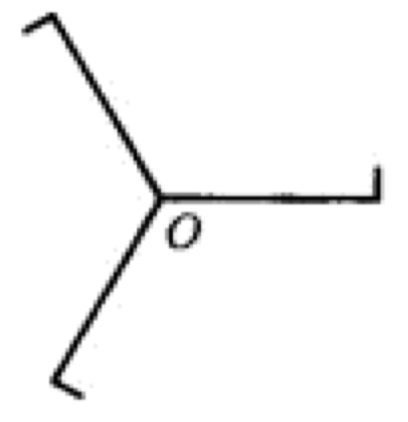
\includegraphics[width=.1\textwidth]{fig/FromLinearEquationToGaloisTheory_RotationExample.png}
\end{figure}
我们用绕O点逆时针转动来描述该图形所具有的对称性:转动$0^\circ$或$360^\circ$记为$g_1$,转动$120^\circ$记作$g_2$,转动$240^\circ$记作$g_3$;对于$g_i, g_i \in G = \{g_1, g_2, g_3\}$,定义$g_j\cdot g_i$表示先进行$g_i$再进行$g_j$,于是$G$是群。

给出对称群的乘法运算如下:
$$
\begin{cases}
g_1 \cdot g_1 = g_1, \quad g_1 \cdot g_2 = g_2, \quad g_1 \cdot g_3 = g_3 \\
g_2 \cdot g_1 = g_2, \quad g_2 \cdot g_2 = g_3, \quad g_2 \cdot g_3 = g_1 \\
g_3 \cdot g_1 = g_3, \quad g_3 \cdot g_2 = g_1, \quad g_3 \cdot g_3 = g_2 \\
\end{cases}
$$

于是得到$G$的乘法表如下,表中第$i$行$j$列的元素是$g_j\cdot g_i$:
\begin{table}[H]
	\centering  % 显示位置为中间
	\caption{standard table}  % 表格标题
	\begin{tabular}{c|c c c}
		& $g_1$ & $g_2$ & $g_3$ \\
		\hline
		$g_1$& $g_1$ & $g_2$ & $g_3$\\
		$g_2$& $g_2$ & $g_3$ & $g_1$\\
		$g_3$& $g_3$ & $g_1$ & $g_2$\\
	\end{tabular}
\end{table}

从表中可以得到一个规律:表中的每一行和每一列都是这三个群元的一个排列。
\end{framed}

\begin{mdframed}[
linecolor=black!40,outerlinewidth=1pt,roundcorner=.5em,innertopmargin=1ex,innerbottommargin=.5\baselineskip,innerrightmargin=1em,innerleftmargin=1em,backgroundcolor=gray!5,
%backgroundcolor=blue!10,%userdefinedwidth=1\textwidth,%shadow=true,%shadowsize=6,%shadowcolor=black!20,%frametitle={The \textit{two-step} model of XMCD:},%frametitlebackgroundcolor=cyan!40,%frametitlerulewidth=10pt
]
\textbf{
重新排列定理:设$g \in G = \{g_1, g_2, \cdots, g_n\}$,则当$i$取遍$, 2, \cdots, n$,$gg_i$或$g_ig$就取遍$G$。
}
\end{mdframed}

\subsection{对称群}
类似于$S_2, S_3, S_4, S_5$,我们把$S_n$定义成$1, 2, \cdots, n$这$n$个数字的置换的全体。接下来定义元素的乘法,使$S_n$成群。为简明起见,以$S_3$为例,对于
$$
g_2 = \begin{pmatrix}
1 & 2 & 3\\1 & 3 & 2
\end{pmatrix}, \quad
g_5 = \begin{pmatrix}
1 & 2 & 3\\2 & 3 & 1
\end{pmatrix}
$$

有
$$
g_2 \cdot g_5 = \begin{pmatrix}
1 & 2 & 3\\1 & 3 & 2
\end{pmatrix} \cdot \begin{pmatrix}
1 & 2 & 3\\2 & 3 & 1
\end{pmatrix}
$$

即
\begin{align*}
  & 1 \xrightarrow{g_5} 2 \xrightarrow{g_2} 3  \\
  & 2 \xrightarrow{g_5} 3 \xrightarrow{g_2} 2  \\
  & 3 \xrightarrow{g_5} 1 \xrightarrow{g_2} 1  \\
\end{align*}

所以
$$
g_2 \cdot g_5 = \begin{pmatrix}
1 & 2 & 3\\3 & 2 & 1
\end{pmatrix} = g_3
$$

不难证明$S_3$在置换的乘法下是群。同样$n$个数字$1, 2, \cdots, n$的全部置换$S_n$,在上述乘法下构成$n!$的\textbf{对称群$S_n$}。

\subsection{子群(subgroup)}
集合有子集合,相应的,群也有子群的概念。
\begin{mdframed}[
linecolor=black!40,outerlinewidth=1pt,roundcorner=.5em,innertopmargin=1ex,innerbottommargin=.5\baselineskip,innerrightmargin=1em,innerleftmargin=1em,backgroundcolor=gray!5,
%backgroundcolor=blue!10,%userdefinedwidth=1\textwidth,%shadow=true,%shadowsize=6,%shadowcolor=black!20,%frametitle={The \textit{two-step} model of XMCD:},%frametitlebackgroundcolor=cyan!40,%frametitlerulewidth=10pt
]
\textbf{
定义:群$G$的非空子集合$H$称为$G$的一个子群,记作$H \unlhd G$,或$G \unrhd H$(原书符号无法打出,类似这样),如果在$G$所定义的乘法运算下,$H$本身构成构成一个群。
}
\end{mdframed}

显然,$\{e\}$和$G$本身都是$G$的子群,它们是$G$的\textbf{平凡子群}。$G$的其它子群则是$G$的\textbf{真子群}。

\begin{framed}
%\verb|\documentstyle[ifthen,12pt,titlepage]{article}|
\small {
例如:对于前文给出的$S_3$:
\begin{align*}
S_3 &= \begin{Bmatrix}
\begin{pmatrix}
1 & 2 & 3\\
1 & 2 & 3
\end{pmatrix}, &
\begin{pmatrix}
1 & 2 & 3\\
1 & 3 & 2
\end{pmatrix}, &
\begin{pmatrix}
1 & 2 & 3\\
3 & 2 & 1
\end{pmatrix}, &
\begin{pmatrix}
1 & 2 & 3\\
2 & 1 & 3
\end{pmatrix}, &
\begin{pmatrix}
1 & 2 & 3\\
2 & 3 & 1
\end{pmatrix}, &
\begin{pmatrix}
1 & 2 & 3\\
3 & 1 & 2
\end{pmatrix}
\end{Bmatrix}  \\
&= \{g_1, g_2, g_3, g_4, g_5, g_6\}
\end{align*}

$H_1 = \{g_1, g_2\}$是一个真子群,$H_2=\{g_1, g_5, g_6\}$也是一个真子群。
}
\end{framed}

设 $H$ 是$G$的一个子群,不难证明$H$的单位元就是$G$的单位元$e$,而且任意$a\in H$在 $H$ 中的逆元就是$a$在$G$中的逆元$a^{-1}$。另外,若要验证$G$的子集$H$对$G$的乘法运算是否成群,就需要判断此时$H$能否满足群的4条公理。不过$G$满足结合律,所以它的子集$H$也满足结合律。因此,只需要验证公理(1)(3)(4)(封闭性、单位元、逆元)。

\begin{mdframed}[
linecolor=black!40,outerlinewidth=1pt,roundcorner=.5em,innertopmargin=1ex,innerbottommargin=.5\baselineskip,innerrightmargin=1em,innerleftmargin=1em,backgroundcolor=gray!5,
%backgroundcolor=blue!10,%userdefinedwidth=1\textwidth,%shadow=true,%shadowsize=6,%shadowcolor=black!20,%frametitle={The \textit{two-step} model of XMCD:},%frametitlebackgroundcolor=cyan!40,%frametitlerulewidth=10pt
]
\textbf{
定理:设 $H \subseteq G$,$H$是$G$的子群的充要条件是对任意$a, b \in H$,有$ab^{-1} \in H$
}
\end{mdframed}

\begin{framed}
%\verb|\documentstyle[ifthen,12pt,titlepage]{article}|
\small{
理解:$H$若想成为$G$的子群,需要满足的条件,是对于任意$a,b \in H$,有$ab^{-1} \in H$,即$a$“乘法运算”$b$的逆得到的元,仍然在$H$中。
}
\end{framed}

子群的概念是重要的,伽罗瓦正式成功地揭示了每一个$n$次多项式都有一个与$S_n$有关的子群——\textbf{该方程的伽罗瓦群}相关联,从而把方程是否根式可解归结为该子群的性质——可解性的研究。在这个意义上,该子群是该方程的“遗传密码”。

\subsection{陪集(cosets)}
现在我们用 $G$的真子群$H$来给出$G$的一个\textbf{分类}。由$H \subset G$,可知存在$a_2 \in G - H$($G$和$H$的差集),于是构造:
$$
a_2H = \{a_2h | h \in H\}
$$

容易证明,$H \cap a_2H = \varnothing$。如果存在$a_3 \in G$,且$a_3 \notin H\cup a_2H$,则同样再构造$a_3H$,也有$a_3H \cap (H \cup a_2H) = \varnothing$。类似地,可得到$a_4H, a_5H, \cdots$,于是当群$G$是有限群时,就有:
$$
G = H \cup a_2H \cup a_3H \cup \cdots a_lH
$$

我们把$G$的具有$aH$形式的子集,称为$G$的关于子群$H$的由元素$a$给出的\textbf{左陪集}。令$a_1 = e$,由$H = eH = a_1H$可知,$H$也是$G$的一个左陪集。于是上式$G = H \cup a_2H \cup a_3H \cup \cdots a_lH$称为$G$的一个\textbf{左陪集分解}。若$|G| = n, |H| = m$,并且把左陪集的个数,称为$H$在$G$中的\textbf{指数},记为$(G:H) = l$,于是考虑到\textbf{每一个左陪集中元素的个数都是$m$},即有:
\begin{mdframed}[
linecolor=black!40,outerlinewidth=1pt,roundcorner=.5em,innertopmargin=1ex,innerbottommargin=.5\baselineskip,innerrightmargin=1em,innerleftmargin=1em,backgroundcolor=gray!5,
%backgroundcolor=blue!10,%userdefinedwidth=1\textwidth,%shadow=true,%shadowsize=6,%shadowcolor=black!20,%frametitle={The \textit{two-step} model of XMCD:},%frametitlebackgroundcolor=cyan!40,%frametitlerulewidth=10pt
]
\textbf{
拉格朗日定理:设 $H$ 是有限群$G$的子群,则$|G| = (G:H)\cdot |H|$
}
\end{mdframed}

\textbf{由上可知,子群$H$的阶$m$是群$G$的阶$n$的一个因子。例如$|S_3| = 6$,所以如果它有子群的话,它只可能有2阶,3阶的真子群,而不可能有4阶,5阶的真子群。}

类似的,我们也有\textbf{右陪集}的概念,这指的是具有:
$$
Ha = \{ha | h \in H\}
$$
形式的集合。

\begin{framed}
%\verb|\documentstyle[ifthen,12pt,titlepage]{article}|
\textbf{关于陪集的定义}:设$(H,\cdot)$是群$(G,\cdot)$的一个子集,$a \in G$,则集合$aH(Ha)$称为由$a$所确定的$H$在$G$中的左陪集(右陪集),简称为$H$关于$a$的左陪集(右陪集),记为$aH(Ha)$。元素$a$称为陪集$aH(Ha)$的代表元素。

(理解,这里的陪集还是属于“子集”的概念,没有要求是“子群”,虽然$H$是$G$的子群,但是$aH$未必要求成群)
~\\

\textbf{关于陪集的定理}:设$H$是$G$的子群,对于任意$a, b \in G$,有:

(1) $aH = bH$ 或者 $aH \cap bH = \varnothing$

(2) $Ha = Hb$ 或者 $Ha \cap Hb = \varnothing$

(来源于:https://www.voicenews.cn/21660.html)

\textbf{对$a$来说的左陪集$aH$, 其实就是$a$在$G$上的一个等价类。}

(来源于知乎:https://zhuanlan.zhihu.com/p/23886266)
\end{framed}

\begin{framed}
%\verb|\documentstyle[ifthen,12pt,titlepage]{article}|
\small{
理解:假如有实数加群$<R, +>$,和一个整数加群$<Z, +>$,则后者一定是前者的子群:
$$
Z = \{\cdots, -n, \cdots, -2, -1, 0, 1, 2, \cdots, n, \cdots \}
$$

我们在实数加群里面随便选取一个$a = 2.5$, 得到$a$确定$G$在$H$上的左陪集是
$$
aH = \{\cdots, 2.5-n, \cdots, 2.5-2, 2.5-1, 2.5, 2.5+1, 2.5+2, \cdots, 2.5+n, \cdots \}
$$

即
$$
aH = \{a+x | x \in Z, a \in R\}
$$

(来源于知乎:https://zhuanlan.zhihu.com/p/23886266)
}
\end{framed}

\subsection{正规子群与商群}

根据$G = H \cup a_2H \cup a_3H \cup \cdots a_lH$,我们定义\textbf{商集合}:
$$
G/H = \{H, a_1H, a_2H, \cdots, a_lH\}
$$

我们希望在$G/H$中引入乘法运算,即\textbf{两个陪集的乘法},使$G/H$成群(理解:$G/H$是“群的群”,因为$G/H$的每个元都是一个子群)。当然,这一乘法应该与$G$的乘法有关联,一个很自然的想法是令:
$$
a_iH \cdot a_jH = (a_i\cdot a_j)H
$$

不过,若$h_i, h_j \in H$,则$a_iH = a_ih_iH, a_jH = a_jh_jH$,即$a_i$与$a_ih_i$都是$a_iH$的代表,$a_j$与$a_jh_j$都是$a_jH$的代表,因此如果上式成立,它应该与代表的选择无关,于是必须有:
$$
a_iH \cdot a_jH = a_ih_iH \cdot a_jh_jH = a_ih_ia_jh_jH
$$

因此应有:
$$
(a_ia_j)H = (a_ih_ia_jh_j)H
$$

然而,对$G$的任意子群$H$来说,这一条件一般是不能满足的。为此,伽罗瓦引入了\textbf{正规子群}这一重要的概念。
\begin{mdframed}[
linecolor=black!40,outerlinewidth=1pt,roundcorner=.5em,innertopmargin=1ex,innerbottommargin=.5\baselineskip,innerrightmargin=1em,innerleftmargin=1em,backgroundcolor=gray!5,
%backgroundcolor=blue!10,%userdefinedwidth=1\textwidth,%shadow=true,%shadowsize=6,%shadowcolor=black!20,%frametitle={The \textit{two-step} model of XMCD:},%frametitlebackgroundcolor=cyan!40,%frametitlerulewidth=10pt
]
\textbf{
正规子群的定义:如果$G$的子群$H$,对任意$a \in G$,满足$aH = Ha$,即此时不必区分左右陪集,则称$H$为$G$的一个正规子群,记作 $G \rhd H$或$H \lhd G$。
}
\end{mdframed}

设$G \rhd H$,由群的乘法定义满足结合律和“重新排列定理”可知,$(a_ih_ia_jh_j)H = (a_ih_ia_j)H =  (a_ih_i)Ha_j =  (a_i)h_iHa_j = a_iHa_j = a_ia_jH$,从而推出了$(a_ia_j)H = (a_ih_ia_jh_j)H$。此时利用$G/H$中的这一乘法,不难证明:
\begin{mdframed}[
linecolor=black!40,outerlinewidth=1pt,roundcorner=.5em,innertopmargin=1ex,innerbottommargin=.5\baselineskip,innerrightmargin=1em,innerleftmargin=1em,backgroundcolor=gray!5,
%backgroundcolor=blue!10,%userdefinedwidth=1\textwidth,%shadow=true,%shadowsize=6,%shadowcolor=black!20,%frametitle={The \textit{two-step} model of XMCD:},%frametitlebackgroundcolor=cyan!40,%frametitlerulewidth=10pt
]
\textbf{
定理:设$G \rhd H$,并按照$a_iH \cdot a_jH = (a_i\cdot a_j)H$定义的元素的乘法,则$G/H$构成群,这个群称为$G$关于正规子群$H$的商群。
}
\end{mdframed}

\begin{framed}
%\verb|\documentstyle[ifthen,12pt,titlepage]{article}|
例:\textbf{可换群$G$的任意子群都是它的正规子群}。

例:若 $H$是$G$的指数为2的子群,则$G = H \cup aH = H \cup Ha$,从而有$aH = Ha$,因此$G \rhd H$。(理解,\textbf{也就是说,如果$H$是$G$的子群,且$H$的指数为2,则$H$就是$G$的正规子群})

例:对任意群$G$而言,群$G$本真与$\{e\}$都是$G$的正规子群,称这两个群为$G$的\textbf{平凡正规子群}。

例:设$G \rhd H$,则 $|G/H| = |G| / |H|$。
\end{framed}

\begin{framed}
%\verb|\documentstyle[ifthen,12pt,titlepage]{article}|
\small {
理解1:把群$G$当成一个高中,里面的元素就是学生。这个高中有三个年级,每个年级5个班,每个班40个学生。

下面来谈谈商的本质,其实\textbf{商就是把有等价关系的两个元素在新的群中看成同一个,而等价关系的给出,就是由被商掉的那个群决定的}。

回到之前的例子,我现在把一个班级看成一个子群,就取高一一班好了,这里的等价关系就是同一个班级的学生是彼此等价的,显然互反性,传递性,对称性满足,这确实是个等价关系。那么做商以后得到的集合是什么呢,这个集合就是这个高中班级的集合,里面有十五个元素:高一一班一直到高三五班。每个元素都是一个集合,里面的元素是这个班级的学生,这样在这个商关系之下,班级也就是所谓的陪集。

现在我们换一下,把年级看成等价关系,被商的子群就是一个年级,就取高一年级,这样得到的商群中的元素就是三个年级。

那么什么是正规子群呢,你可以把正规子群理解为一类特殊的子群,特殊在于,
\textbf{商掉正规子群得到的商群有自然的群结构}。在上面的例子中,可以非常不严格的把班级和年级看成正规子群,因为它们是特殊的,因为生活中我们常以班级年级作为统一的单位。

在上面的例子中,还有什么可以当子群呢,你不妨把学号为1的学生全体当一个子群,此时的等价关系就是相同的学号。这样得到的商群就是40个,为什么我要把它当子群,因为在生活中你基本遇不到学校以学号来划分全体学生…在正规子群这里,类比是很不贴切的,我主要想告诉你的是正规子群是极其特殊的子群。

来源于知乎:https://www.zhihu.com/question/63046350/answer/204840915
~\\

理解2:一个群可以看作正规子群和商群“组合”起来的(在特殊情况下就是直积),这样就把复杂的群化解成了简单的群,得到一个群的合成因子。

来源于知乎:https://www.zhihu.com/question/21561484/answer/92539982
~\\

理解3:回忆,\textbf{商集合}是由集合$A$的各个类作元素得到的集合,其中的每个类都是一个等价类(即类内元素等价);而\textbf{商群}是由正规子群构成的群。

理解4:再加深一下对“商”的理解,比如有6个桔子,按照每行2个排列成3行,那么对于每一行的2个桔子,可以看成这一行内的桔子是等价的,并且一共有3“类”。
}
\end{framed}

\subsection{循环群(cycle group)与$n$次本原根}
设$G$是一个群,而$e$是它的单位元。我们对于$0 \in N, n \in N^*$,规定 $a^0 = e, a^n = \underbrace{a\cdot a \cdot \cdots \cdot a}_{n\text{个}}$,$a^{-n} = (a^{-1})^n$,则显然有$a^m \cdot a^n = a^{m+n}, (a^n)^m = a^{nm}, \forall m, n \in \mathbf{Z}$。

因此,我们引入\textbf{循环群}的定义:
\begin{mdframed}[
linecolor=black!40,outerlinewidth=1pt,roundcorner=.5em,innertopmargin=1ex,innerbottommargin=.5\baselineskip,innerrightmargin=1em,innerleftmargin=1em,backgroundcolor=gray!5,
%backgroundcolor=blue!10,%userdefinedwidth=1\textwidth,%shadow=true,%shadowsize=6,%shadowcolor=black!20,%frametitle={The \textit{two-step} model of XMCD:},%frametitlebackgroundcolor=cyan!40,%frametitlerulewidth=10pt
]
\textbf{
循环群的定义:对于$n$阶群$G$,如果存在$a \in G$,使得$G = \{a^0, a, a^2, \cdots, a^{n-1}\}$,则称$G$为由$a$生成的(有限)循环群,记作$G = \langle a \rangle$,$a$是$G$的一个生成元。
}
\end{mdframed}

对于有限群$G$,取任意$a \in G$,$a \neq e$,构造 $H = \langle a \rangle$,不难证明$H$是$G$的一个循环子群。\textbf{如果$G$是素数阶的,则由拉格朗日定理可知,$G$不含任何真子群,因此$G = H = \langle a \rangle$,即
$G$是循环群,当然也是可换群,并且它的每一个非单位元都是生成元。}

\begin{framed}
%\verb|\documentstyle[ifthen,12pt,titlepage]{article}|
例:根据前文定义的模$n$同余类集合$Z_n$和同余类乘群$Z'_n$,即:
$$
\bar{a} = \{a + kn\ | k \in Z\}
$$
$$
Z_n = \{\bar{1}, \bar{2}, \cdots, \bar{n}\}
$$
$$
Z'_n = \{\bar{k} \in Z_n | 1 \le k \le n, (k,n) = 1\}
$$

有:$Z'_3 = \{\bar{1}, \bar{2}\} = \langle\bar{2}\rangle $;同理,$Z'_5 = \{\bar{1}, \bar{2}, \bar{3}, \bar{4}\} = \langle\bar{2}\rangle$;$Z'_7 = \{\bar{1}, \bar{2}, \bar{3}, \bar{4}, \bar{5}, \bar{6}\} = \langle\bar{3}\rangle$。

理解:根据前文,我们知道$Z_n$和$Z'_n$上定义的乘法运算是$\overline{a}\cdot \overline{b} = \overline{ab}$,并且知道$Z_n$不是群(因为它的元$\overline{n}$没有逆元),并且$Z'_n$是群。

因此我们知道,对于群$Z'_n$来说,$\bar{1}$是它的单位元。那么对于任意元素$a \in G, a \neq e$,并且如果$Z'_n$是素数阶的,那么$Z'_n$的每一个非单位元都是生成元。

\textbf{
理解:注意,$Z'_n$是素数阶的,不等价于$n$是素数;比如$Z'_5 = \{\bar{1}, \bar{2}, \bar{3}, \bar{4}\} $,5是素数,但是$|Z'_5| = 4$ 不是素数,因此不能推导出来 $Z'_5$的任意非单位元$\bar{2}, \bar{3}, \bar{4}$都是它的生成元,实际上,$\bar{4}$就不是$Z'_5$的生成元($\bar{4}$ 只能循环生成 $\bar{1}$ 和 $\bar{4}$)。
}
\end{framed}

\begin{mdframed}[
linecolor=black!40,outerlinewidth=1pt,roundcorner=.5em,innertopmargin=1ex,innerbottommargin=.5\baselineskip,innerrightmargin=1em,innerleftmargin=1em,backgroundcolor=gray!5,
%backgroundcolor=blue!10,%userdefinedwidth=1\textwidth,%shadow=true,%shadowsize=6,%shadowcolor=black!20,%frametitle={The \textit{two-step} model of XMCD:},%frametitlebackgroundcolor=cyan!40,%frametitlerulewidth=10pt
]
\textbf{
一般地,当$p$是素数时,可以证明$Z'_p = \{\overline{1}, \overline{2}, \cdots, \overline{p-1}\}$是循环群。  
}
\end{mdframed}

\begin{framed}
%\verb|\documentstyle[ifthen,12pt,titlepage]{article}|
\small {
理解:以模6加法群$\langle Z6, +\rangle$入手,来认识循环群的特点。

首先,循环群,顾名思义,cycle group即带有循环的意思。怎么个循环法呢?

我们看$\langle Z6, +\rangle$中的元素$\{0,1,2,3,4,5\}$。取其中的元素1,不停地对自身进行模6加法,即对本身进行幂运算。可得:
\begin{align*}
& 1^1=1 \\
& 1^2=1+1=2 \\
& 1^3=1+1+1=3 \\
& 1^4=1+1+1+1=4 \\
& 1^5=1+1+1+1+1=5 \\
& 1^6=1+1+1+1+1+1=0 \text{(模6加法意义下)}\\
& 1^7=1+1+1+1+1+1+1=1\text{(模6加法意义下)} \\
& \cdots
\end{align*}

如上对1不断幂运算,可见两个现象:

1、可以遍历所有的元素,也可以说,我们仅用元素1就能生成所有的元素,这就是循环群里的生成元的概念。

2、幂运算的结果就是123450123450123450这样不断的循环,这就是循环群名字由来。

现在,我们继续思考,如果对其它元素进行不断的幂运算呢,会出现什么结果?

经过不断的幂运算,我们发现:元素0形成的结果只有0,结果集合为\{0\};元素2、4形成的结果是一样的,结果集合为\{0,2,4\};元素3形成的结果集合为\{0,3\};元素1、5形成的结果为\{0,1,2,3,4,5\};可见,不同的元素,有的形成的结果不同,有的却相同。我们可以按照他们生成的结果来将他们划分为不同的群体。

对于元素1、5,他们都能生成所有元素,所以他们两个元素不仅证明了这个群是循环群,还说明他们都是循环群的生成元。他们生成了\{0,1,2,3,4,5\}这个子群(或者说群本身,也叫平凡子群)并且他们都是6阶元素,所谓6阶,就是$a^6=e=0$(幺元,或称单位元,这个群的单位元是0)。6阶也是这个群的阶数。

对于元素2、4,他们生成了子群\{0,2,4\},他们都是3阶元素。

对于元素3,生成了子群\{0,3\},他是2阶元素。

对于元素0,生成了子群\{0\},他是1阶元素。

通过对上面的观察,我们又看出一些规律,就是:

(1). n阶元素生成的子群中具有n个元素

(2). 一个n阶群,他具有p个不同类型的生成子群,p是n的正因子个数,比如本例中6的正因子有1,2,3,6共四个。

(3). 一个n阶群,他的生成元个数是小于n且与n互为素数的个数。本例中,小于6且与6互素的数是1、5,共两个,所以这个群的生成元就正好2个。

(来源:https://blog.csdn.net/u013709443/article/details/82823678)
}
\end{framed}

在之前的章节中,我们研究过$x^n - 1 = 0$的解集合为:
$$
1, \zeta = e^{i2\pi/n}, \zeta^2 = e^{i4\pi/n}, \cdots,  \zeta^{n-1} = e^{i2\pi(n-1)/n}
$$

(在复平面中,这$n$个根$1, \zeta, \zeta^2, \cdots, \zeta^{n-1}$均匀地分布在圆心为点 $O$,半径为 1 的一个圆上)

即方程 $x^n-1=0$的解集合$G_n = \{1, \zeta, \cdots, \zeta^{n-1}\}$,其中$\zeta = e^{i2\pi/n}$。对于集合$G_n$,以数的乘法为$G$中元素的乘法,显然$G_n$是一个$n$阶循环群,且$\zeta$是它的一个生成元。

由其中的元的性质可知,$G_1 = \{1\} = \langle 1 \rangle$,$G_2 = \{1, -1\} = \langle -1 \rangle$,$G_3 = \{1, \omega, \omega^2\} = \langle \omega \rangle = \langle \omega^2 \rangle$,$G_6 = \{1, \zeta, \omega, -1, \omega^2, \zeta^5\} = \langle \zeta \rangle = \langle \zeta^5 \rangle$。由此看见,$x^6-1=0$的6个根中,只有$\zeta, \zeta^5$是$G_6$的生成元,而其它的4个根都不是$G_6$的生成元。

因为$1, -1, \omega, \omega^2$满足的$x^n-1=0$型的方程的最低次数分别为:$n = 1, 2, 3$,它们只能分别是$G_1, G_2, G_3$的生成元。因此,我们把$1, -1, \omega, \omega^2$分别称为1次,2次和3次\textbf{本原根},即是这些方程所“固有的”根。按照这种说法,$\omega, \omega^5$就是6次本原根了。

上面从是否是$G_6$的生成元的角度,把$x^6-1=0$的根分成了两类:非本原根和本原根。注意到 $\zeta^6=1, \zeta^2, \zeta^3, \zeta^4$ 这4个非本原根中的指数6, 2, 3, 4 与$n=6$都不是互素的,因此不难得出本原根的另一种刻画:$\zeta^k$是$x^6 - 1 = 0$的一个本原根,当且仅当$(k,6) = 1$。

在一般情况下,$x^n-1=0$的解$1, \zeta, \cdots, \zeta^{n-1}$中,凡满足$(k,n) = 1$的$k$所确定的根$\zeta^k$是$G_n$的生成元,是$x^n-1=0$的本原根,称为\textbf{$n$次本原根}。因此,$x^n-1=0$的本原根共有$\varphi(n)$个。当$n=$素数$p$时,$\varphi(p) = p - 1$,即$\zeta, \cdots, \zeta^{p-1}$都是本原根。

于是在$x^6-1=0$的6个根中:
\begin{itemize}
\setlength{\itemsep}{0pt}
\setlength{\parsep}{0pt}
\setlength{\parskip}{0pt}
	\item 1次本原根有$\varphi(1) = 1$个:1;
	\item 2次本原根有$\varphi(2) = 1$个:-1;
	\item 3次本原根有$\varphi(3) = 2$个:$\omega, \omega^2$;
	\item 6次本原根有$\varphi(6) = 2$个:$\zeta, \zeta^5$;
\end{itemize}

因此,$6 = \varphi(1) + \varphi(2) + \varphi(3) + \varphi(6) = \sum_{d|6}\varphi(d)$,其中$\sum$是求和符号,下标$d|6$表示,对$\varphi(d)$的求和时,$d$取遍6 的所有因子,即$d = 1, 2, 3, 6$。而在一般情况下,有:
$$
\sum_{d|n} \varphi(d) = n
$$

\subsection{单群}
\begin{mdframed}[
linecolor=black!40,outerlinewidth=1pt,roundcorner=.5em,innertopmargin=1ex,innerbottommargin=.5\baselineskip,innerrightmargin=1em,innerleftmargin=1em,backgroundcolor=gray!5,
%backgroundcolor=blue!10,%userdefinedwidth=1\textwidth,%shadow=true,%shadowsize=6,%shadowcolor=black!20,%frametitle={The \textit{two-step} model of XMCD:},%frametitlebackgroundcolor=cyan!40,%frametitlerulewidth=10pt
]
\textbf{
单群的定义:如果群$G$除了$G$本身和$\{e\}$这两个平凡的正规子群外,不含任何其他的正规子群,则称$G$为(简)单群。
}
\end{mdframed}

素数阶群必是可换群,又因为它没有任何真子群,所以它又是可换单群;反过来,设$G$是$n$阶可换单群,因此$G$就没有任何真子群,任取$a \in G$,且$a \neq e$,构造$\langle a \rangle$,那么$\langle a \rangle = G$,于是$G = \{a^0=e, a, a^2, \cdots, a^{n-1}\}$;若 $n$是合数,则从$n = l \cdot m, 1 < l < n, 1 < m < n$ 可推知$\langle a^l \rangle$ 是$G$的一个真子群,这就矛盾了,因此$n$比是素数。所以\textbf{有限可换单群}一定是素数阶群。

\subsection{群的同态映射与同构映射}

%\printbibliography
\bibliography{../../ref}
\bibliographystyle{plain}
\end{document}